% Figure from MATH 591 notes, section 72 (Lecture 27). From the board (Lecture 27): U and its image under the flow.
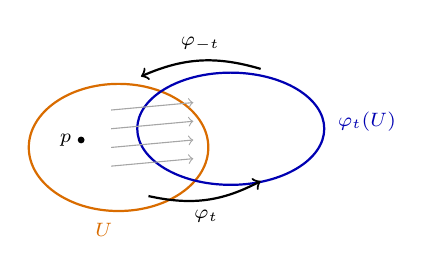
\begin{tikzpicture}[scale=0.95]
\draw[thick, orange!85!black] (0,0) ellipse (1.2 and 0.85); \node[orange!85!black, font=\scriptsize] at (-0.2,-1.1) {$U$};
\draw[thick, blue!70!black] (1.5,0.25) ellipse (1.25 and 0.75); \node[blue!70!black, font=\scriptsize, anchor=west] at (2.8,0.35) {$\varphi_t(U)$};
\fill (-0.5,0.1) circle (1.3pt) node[left, font=\scriptsize] {$p$};
\foreach \y in {-0.25,0.0,0.25,0.5} { \draw[->, gray!70] (-0.1,\y) -- (1.0,\y+0.1); }
\draw[->, thick] (0.4,-0.65) to[bend right=20] node[below, font=\scriptsize] {$\varphi_t$} (1.9,-0.45);
\draw[->, thick] (1.9,1.05) to[bend right=20] node[above, font=\scriptsize] {$\varphi_{-t}$} (0.3,0.95);
\end{tikzpicture}
